\chapter{Mediciones y Resultados}
Se conectan entonces ambos circuitos en la placa \textit{Electronics Explorer}. Debido a las limitaciones del dispositivo, se utilizó una tension de alimentacion de $V_{CC} = 9V$ tanto para el par Darlington como para la carga activa.
A su vez se utiliza el generador arbitrario de funciones para inyectar una señal de $500 mV$ a una frecuencia de $10kHz$ con el objetivo de medir la respuesta del circuito a pequeñas señales. En principio se plantea una senal de $50 mV$, pero debido a una considerable cantidad de ruido en la medicion se imposibilita la medicion precisa del sistema.
Requiriendo entonces una mayor entrada, esta se incrementa cuidando no perder la linealidad de la respuesta hasta el valor propuesto previamente.
La medición de la ganancia de corriente no es realizable. Principalmente debido a que la corriente de entrada es menor de la medible con el equipo previsto, sin afectar el comportamiento del circuito.

\section{Circuito Construido}
El circuito realizado se encuentra en la figura REFERENCIA. En donde se alterna en el emisor de $Q2$ entre dos resistencias en serie representando $R_E$ y en la fuente de corriente espejo conformado por los MOS-FET del lado derecho.

INSERTAR FOTO


\section{Mediciones}
A continuacion se presentan las mediciones de los parametros presentados previamente de manera teorica. Tanto para el Darlington con carga activa y carga pasiva.

\subsection{Caracterización de fuente de corriente}

Es necesario en principio encontrar el valor de $I_O$ de la fuente de corriente. Al ser un componente real, no se puede esperar que ambos transistores n-MOS compartan el mismo valor de $\frac{W}{L}$, por lo que la relacion de corrientes escrita en \ref{eq:io func iref} no es unitaria.
Como se requiere un valor especifico de $I_O$ para la experiencia, se utiliza una resistencia variable como $R_{ref}$ y se la varia hasta que en la salida la corriente sea de los $8,6 mA$ requeridos.

\subsection{Polarización con Carga Pasiva}

Para verificar el correcto funcionamiento del par Darlington, y su correspondencia con la teoria, se realizan mediciones de la polarizacion del mismo. Caracterizada por la tabla REFERENCIA.



\subsection{Ganancia de Tensión}

En la tabla \ref{table:comp av} se muestran los resultados para $\Delta_V$ y $\Delta_{Vs}$ en ambas configuraciones. Y en contraste con los simulado y lo esperado teoricamente.



\begin{table}[ht]
    \centering
    \begin{tabular}{|l|l|l|l|}
    \hline
    $\Delta_V $  & Medida   & Teorica  & Simulacion \\ \hline
    Carga Pasiva & $0.967$  & $0,9904$ &  $XX$       \\ \hline
    Carga Activa & $0.992$  & $0,9992$ &  $XX$          \\ \hline
    \end{tabular}
    \caption{Tabla comparación $\Delta_V$}\label{table:comp av}
\end{table}

También se observan en las figuras REFERENCIAS, el contraste entre formas de onda de salida y entrada para ambas cargas.


%%\begin{figure}[H]
    %%\centering
    %%\includegraphics[width=.45\textwidth]{figs/Rauch/Histogramas/Histograma f0.png}
    %%\includegraphics[width=.45\textwidth]{figs/Rauch/Histogramas/Histograma B.png}
    %%\caption{Histogramas para frecuencia central y ancho de banda normalizado}
  %%  \label{fig:histo f0 y B BP}
%%\end{figure}

\begin{figure}[ht]
\begin{subfigure}{.45\textwidth}
  \centering
  % include first image
  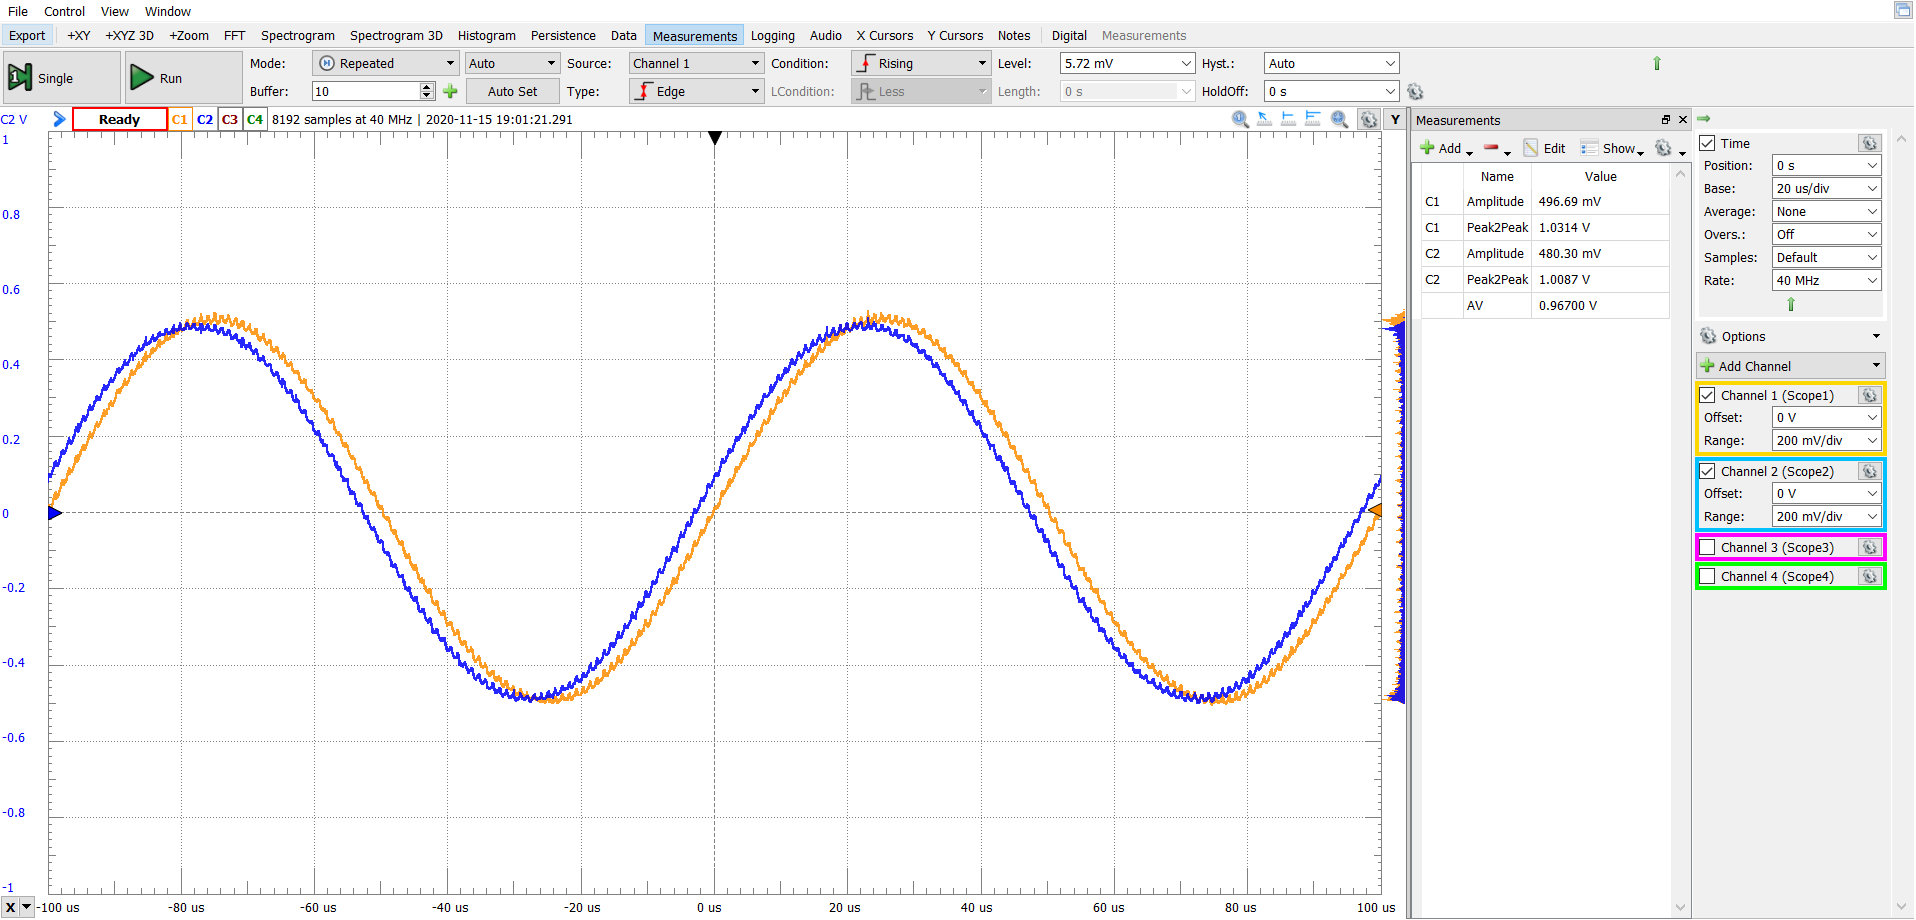
\includegraphics[width=.8\linewidth]{4_medicion/figs/2 pasada/Pasiva/carga pasiva Av c1 entrada c2 salida.png}  
  \caption{Carga Pasiva}
  \label{fig:Av carga pasiva}
\end{subfigure}
\begin{subfigure}{.45\textwidth}
  \centering
  % include second image
  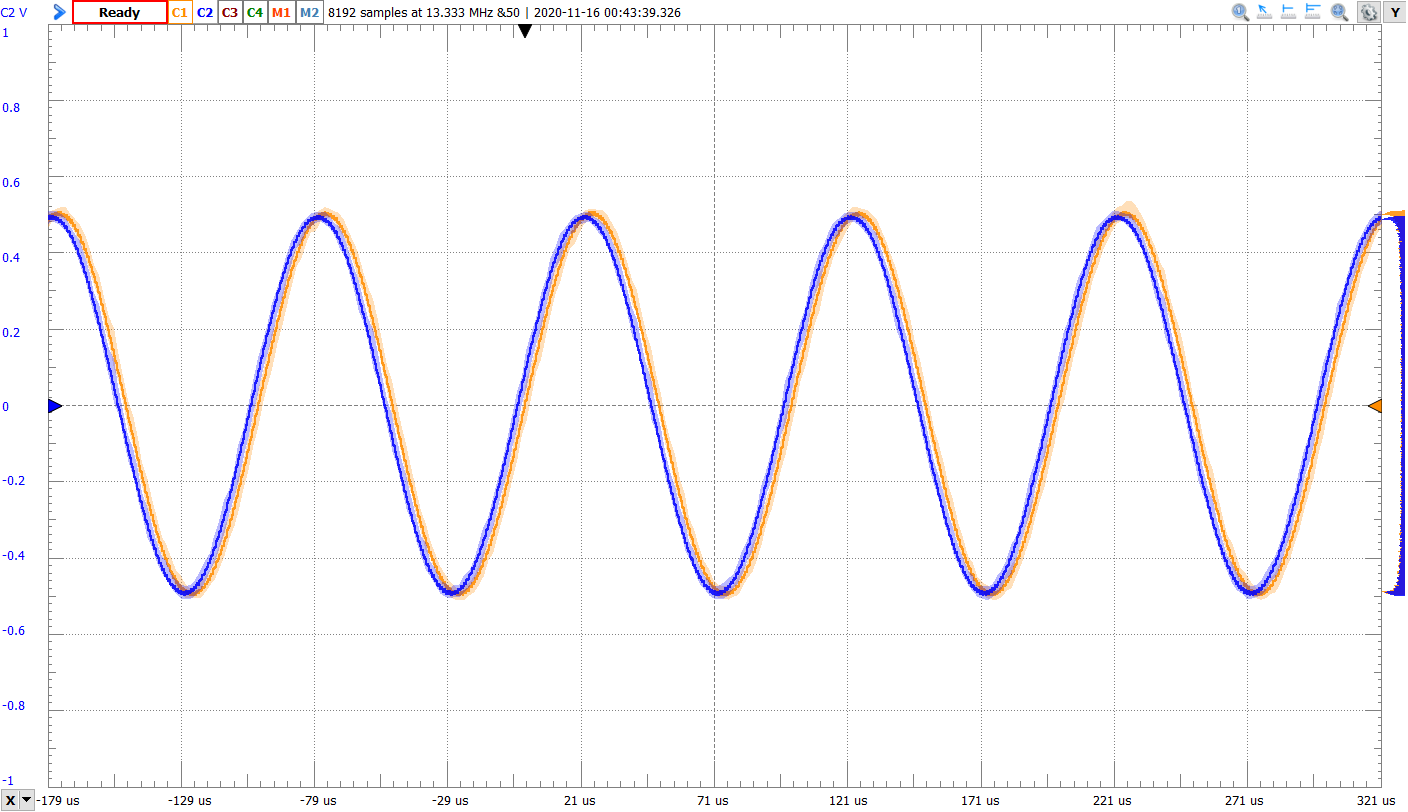
\includegraphics[width=.8\linewidth]{4_medicion/figs/2 pasada/Activa/carga activa Av c1 entrada c2 salida.png}  
  \caption{Carga Activa}
  \label{fig:Av carga activa}
\end{subfigure}
\caption{Adquisición Osciloscopio}
\label{fig:Av oscilo}
\end{figure}

\subsection{Impedancias de Entrada y Salida}

El procedimiento que se emplea para medir la impedancia de entrada consta en insertar una resistencia de referencia de $1 k\Omega$ con tolerancia $1\%$entre el generador de ondas y el capacitor de desacople en la base de $Q1$. Se elige este valor ya que es comparable al esperado teoricamente (ESTO NOSE BIEN GUITARREARLO).
Midiendo la caida de tension en esta y dividiendo por su valor nominal, se haya la corriente que entra a la base del transistor para pequenias seniales. Luego el cociente entre la tension de entrada a la base, y la corriente previamente calculada se estima la impedancia de entrada.
Se realiza el mismo procedimiento para las dos cargas, por mas que se espera un resultado muy similar. En la tabla REFERENCIA, se contrasta lo medido,simulado y calculado teoricamente.

\begin{table}[ht]
    \centering
    \begin{tabular}{|l|l|l|l|}
    \hline
    $r_{ia}$     & Medida       & Teórica         & Simulación \\ \hline
    Carga Pasiva & $1013\Omega$ & $1000\Omega $   &  $XX $          \\ \hline
    Carga Activa & $1018\Omega$ & $1000\Omega $  &  $XX $          \\ \hline
    \end{tabular}
    \caption{Comparación impedancia de entrada}\label{table:Ri comp}
\end{table}

Para la impedancia de salida se realiza una tecnica prevista en el material didactico de la catedra. Consta en medir la tension a la salida del amplificador a circuito abierto (carga infinita),denominada $V_{open}$. Luego se introduce una carga $R_L$ y se mide la tension $V_L$ a traves de la misma.
Contando con estos valores se emplea la ecuacion \ref{eq:zout teor}, encontrando asi un valor para la impedancia de salida.

\begin{equation}
    R_O = R_L(\frac{V_{open}}{V_L}-1)
    \label{eq:zout teor}
\end{equation}

\begin{table}[ht]
    \centering
    \begin{tabular}{|l|l|l|l|}
    \hline
    $r_{oa}$     & Medida     & Teórica         & Simulación \\ \hline
    Carga Pasiva & $23\Omega$ & $5,91\Omega $   &  $XX $          \\ \hline
    Carga Activa & $18\Omega$ &  $5,91\Omega $  &  $XX $          \\ \hline
    \end{tabular}
    \caption{Comparación impedancia de Salida}\label{table:Ro comp}
\end{table}

\subsection{Respuesta en Frecuencia}

La respuesta en frecuencia se mide haciendo uso del \textit{Network Analizer} incluido en el equipo de medicion. Debido a su bajo ancho de banda se dificulta medir el polo de alta, ya que el limite de medicion se impone a los $10 MHz$. No obstante una decada antes del polo previsto se comienza a ver un cambio de fase, como es de esperar.
El polo de baja se observa claramente en el rango determinado. En el grafico REFERENCIA se muestra la respuesta medida.

\begin{figure}[ht]
    \begin{subfigure}{.45\textwidth}
      \centering
      % include first image
      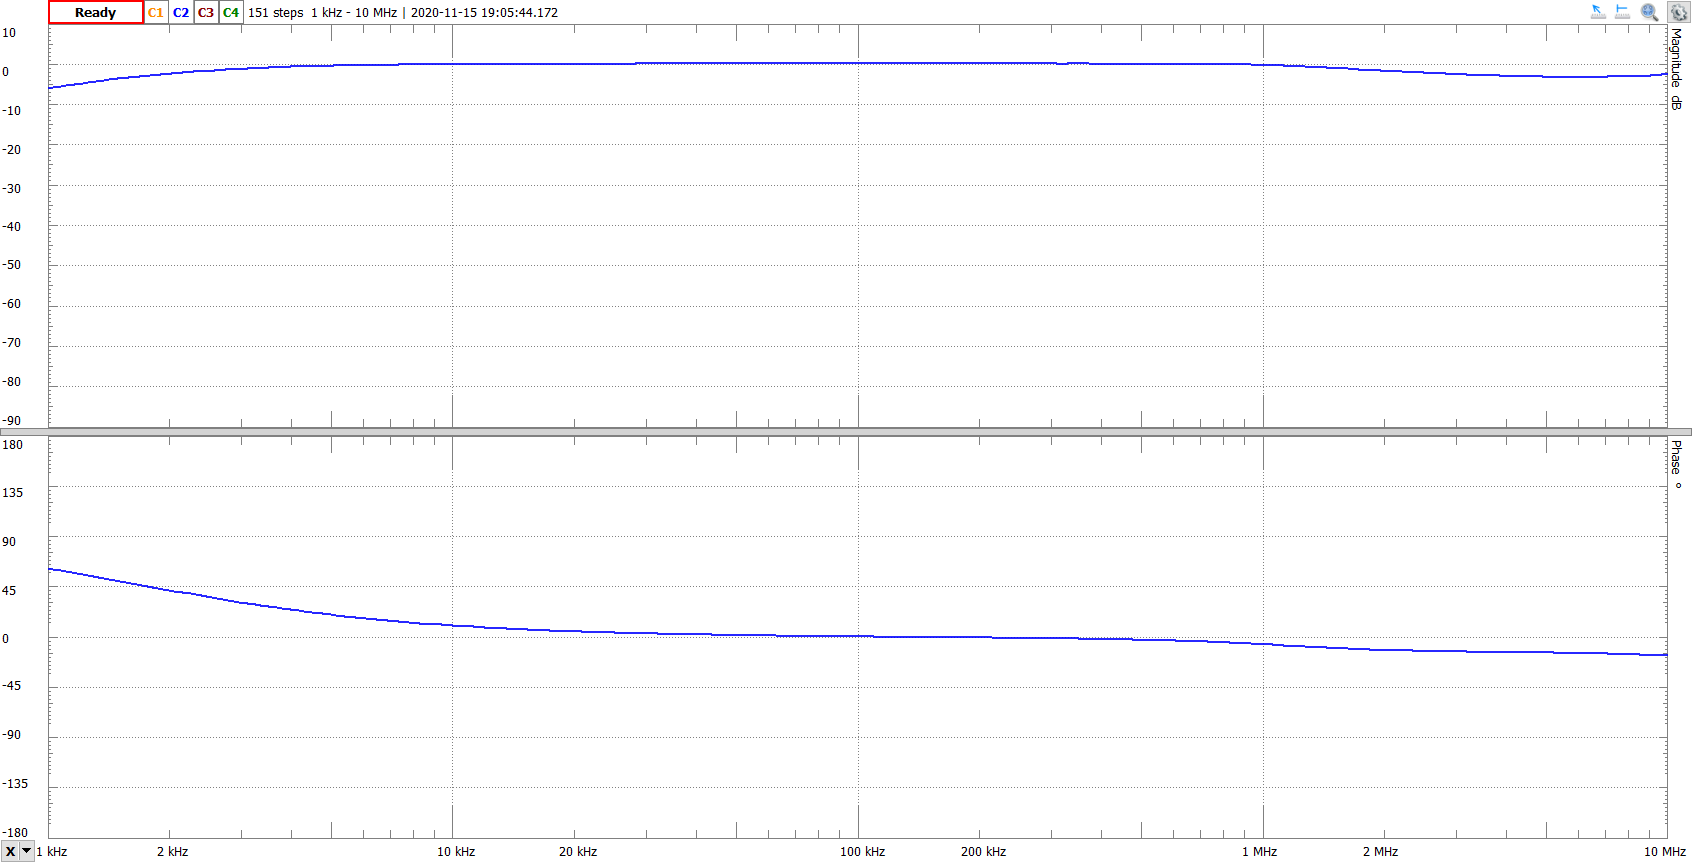
\includegraphics[width=.8\linewidth]{4_medicion/figs/2 pasada/Pasiva/resp frec.png}  
      \caption{Carga Pasiva}
      \label{fig:frec carga pasiva}
    \end{subfigure}
    \begin{subfigure}{.45\textwidth}
      \centering
      % include second image
      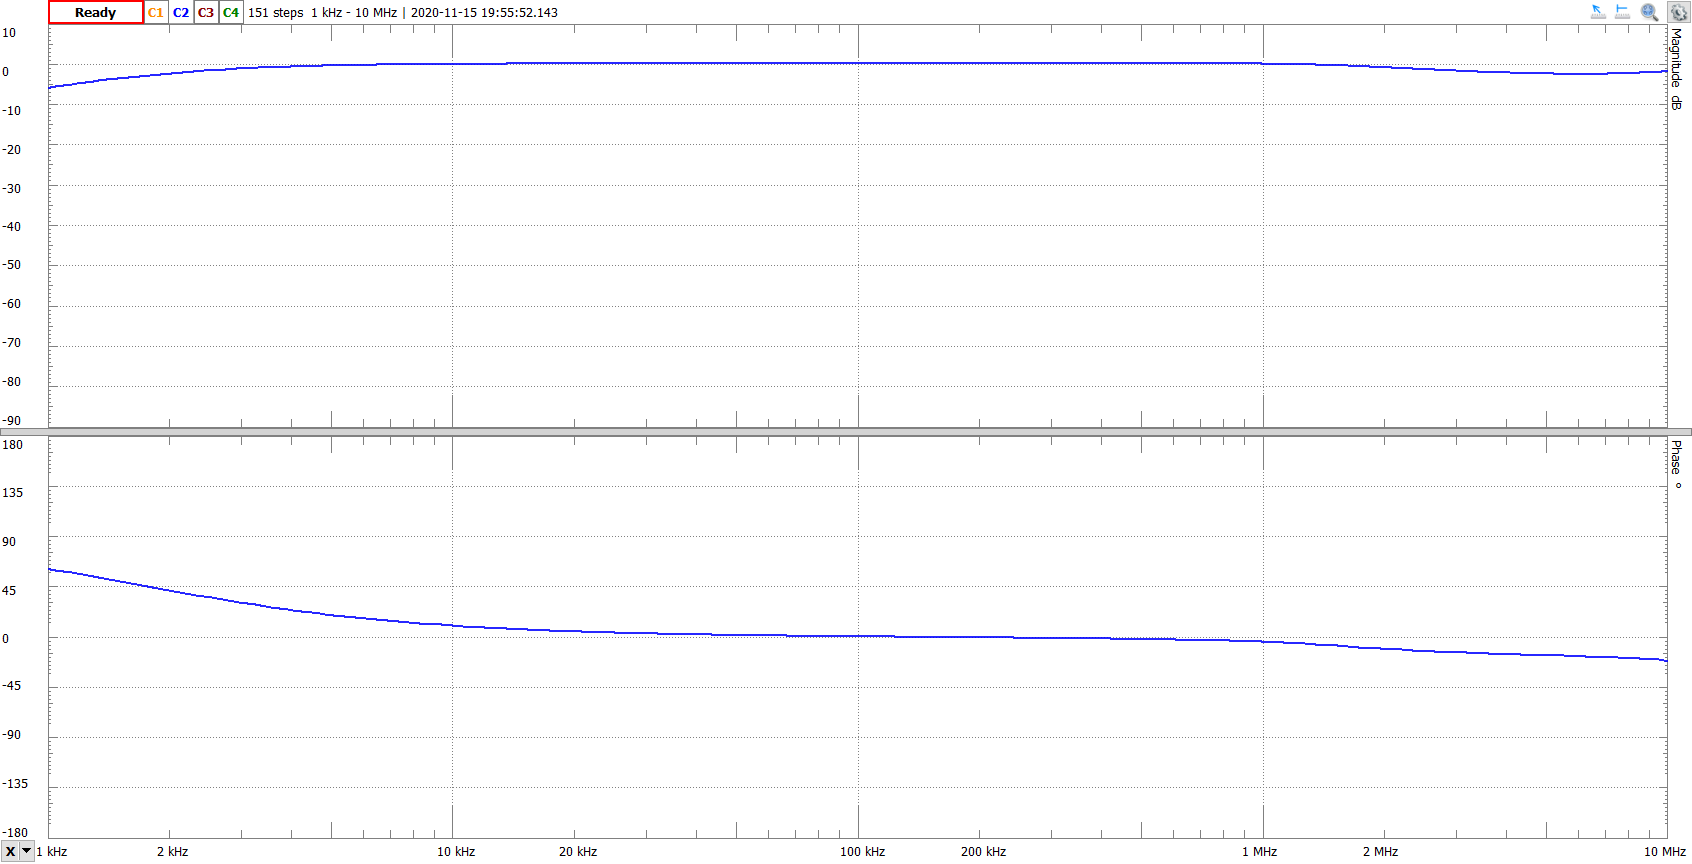
\includegraphics[width=.8\linewidth]{4_medicion/figs/2 pasada/Activa/respfrec.png}  
      \caption{Carga Activa}
      \label{fig:frec carga activa}
    \end{subfigure}
    \caption{Respuesta en frecuencia}
    \label{fig:resp frec oscilo}
    \end{figure}




